% !TeX root = ../../msc-thesis.tex
\documentclass[../../msc-thesis.tex]{subfiles}

\begin{document}

\section{Indirect composition control of a C3 Splitter column}

The second example to be tested in \mtc consists is a particular case of \soc 
structure selection: Indirect control. As stated before \cite{Hori2005}, 
indirect control consists when, for some reason, one is unable to control 
directly one or more variables (denominated by \textcite{Hori2005} as 
``primary'' variables), and consequently tries to control a set of 
``secondary'' variables, that will (hopefully) maintain the ``primary'' ones 
at their desired setpoints. As demonstrated in the past 
\cite{Hori2005,Alstad2009}, the selection of a control structure for 
indirect control is a special case of the exact local method derived by 
\textcite{Halvorsen2003} and that had an explicit solution derived by 
\textcite{Alstad2009}. 

In order to use the exact local method for the special case of indirect 
control, the control strucutre designer must only impose a objective 
function that will minimize the error between the ``primary'' variables and 
their desired setpoints. In fact, this approach has been successfully done 
previously \cite{Hori2008}. As mentioned before, \mtc uses the exact local 
method with explicit solution from \textcite{Alstad2009} to report to the 
user the best sets of controlled variables with \soc properties. 

A didactic case of indirect control 
that happens on the industry consists in composition control of distillation 
columns. Due to unreliability and slow dynamics of online analyzers, the 
direct control of compositions becomes infeasible, or at least, very 
difficult to be done. On the other hand, the market demand and/or 
environmental legislation will, very often, impose purity levels to key 
components at the distillation columns. Therefore, there is a conflict 
between process instrumentation and market/environmental restrictions. 

The case used as the second test-bed in \mtc derives directly from a 
previous work of the author \cite{Alves2018}, which is a propylene-propane 
splitter, being depicted in \autoref{fig:c3splitterflowsheet}. The previous 
publication from \textcite{Alves2018} showed that, from an economic plantwide 
control perspective, the best set of controlled variables to be chosen 
would be the composition of propene at the top stream and the composition 
of propene lost at the bottoms stream, as can be seen in 
\autoref{eq:setc3splitter}.

\begin{figure}[htb]
    \centering
    \caption{C3 Splitter Column Process flowsheet}
    \label{fig:c3splitterflowsheet}
    \makebox[1.0\textwidth]{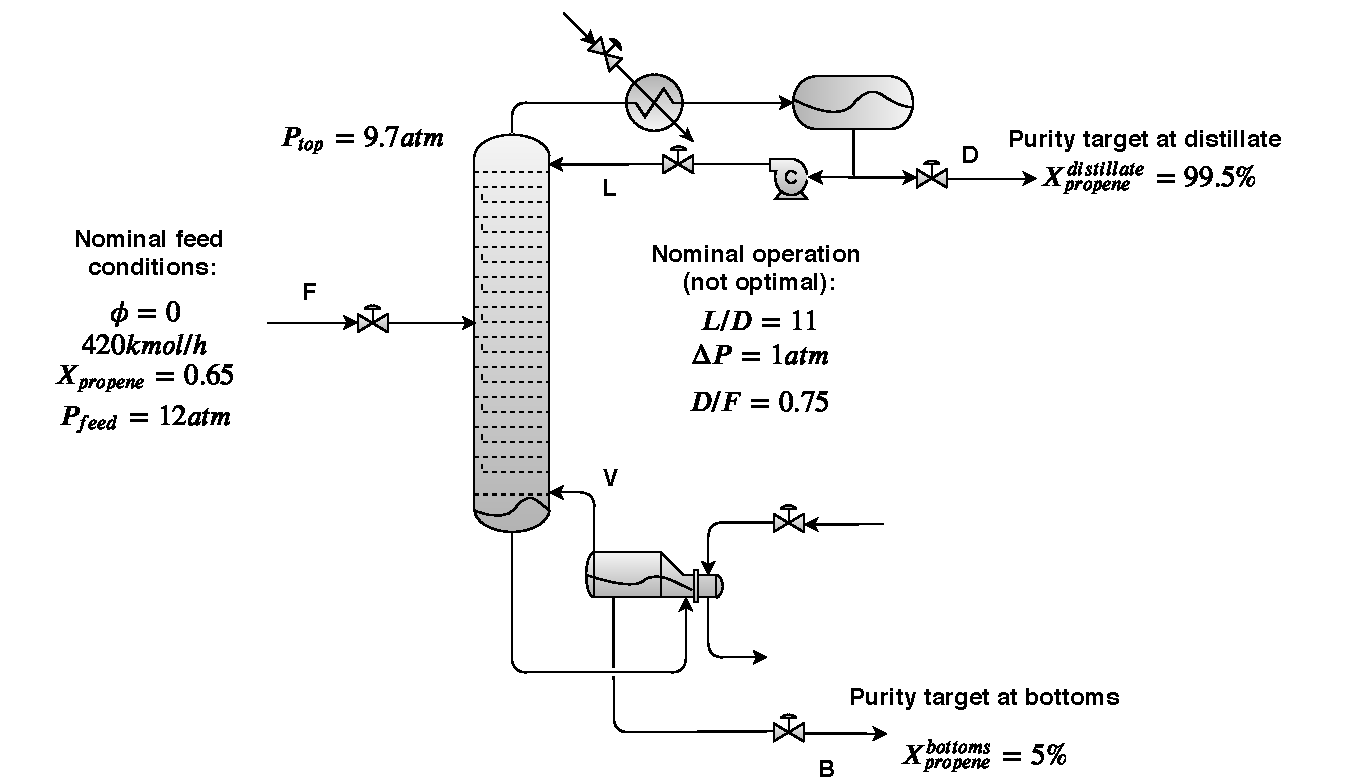
\includegraphics[width=1.0\textwidth]
    {c3splitter2.pdf}}
\end{figure}

\begin{equation}
    c=\left(\begin{array}{c}
        {x_{top}^{propene}} \\
        {x_{bottom}^{propene}}
        \end{array}\right)
    \label{eq:setc3splitter}
\end{equation}

Given the fact that the cited control structure uses two compositions 
measurements that are difficult to be directly controlled, \mtc will be used 
to find a \soc structure for this problem. The objective function in question 
will be the relative steady-state deviation \cite{Hori2008} from the nominal 
optimal setpoint found by \textcite{Alves2018}, depicted in 
\autoref{eq:indirectindex}.

\begin{equation}
    \Delta x^2 = \left(\frac{x_{\text {top }}^{\mathrm{propene}} 
    -x_{\text {setpoint}}^{\mathrm{propene}}}
    {x_{\text {setpoint}}^{\mathrm{propene}}}\right)^{2}
    +\left(\frac{x_{\text {bottom }}^{\mathrm{propene}}
    -x_{\text {setpoint}}^{\mathrm{propene}}}
    {x_{\text {setpoint}}^{\mathrm{propene}}}\right)^{2}
    \label{eq:indirectindex}
\end{equation}

The economically optimal values for the setpoints at the top and bottom 
streams of the C3 splitter are 0.995 (active constraint for economic 
plantwide control problem) and 0.05, respectively. For the latter, the 
setpoint was rounded to 0.05. The constraint that exists in this problem 
regards the reboiler duty, unable to surpass the limit of 80 $GJ/h$. 
The economically optimal values for the compositions and the reboiler 
duty constraint are taken from \textcite{Alves2018}.

\begin{itemize}
    \item C-1: Reboiler duty $\leq 80 GJ/h $
\end{itemize}

The main process disturbances considered are the same from 
\textcite{Alves2018}:

\begin{itemize}
    \item D-1: Propylene flow rate
    \item D-2: Propane flow rate
    \item D-3: Feed vapor fraction $\phi$
\end{itemize}

The number of degrees of freedom for this process is two 
\cite{Alves2018,Skogestad2000} and without loss of generality, they are the 
same from \textcite{Alves2018}:

\begin{enumerate}
    \item Reflux ratio
    \item Distillate to feed ratio
\end{enumerate}

The distillation column studied has 146 stages. As \textcite{Alves2018} did, 
to test the \soc theory, some temperature measurements will be selected by the 
slope criterion \cite{Luyben2006} as promising CV candidates and will also 
choose (based on the same criterion) poor candidates. To illustrate, 
the temperature profile for the C3 splitter is shown in 
\autoref{fig:c3splittertprofile}. In addition, several flows and flow ratios 
were considered as CV candidates to be tested.

\begin{figure}[htb]
    \centering
    \caption{C3 Splitter Column - Temperature profile.}
    \label{fig:c3splittertprofile}
    \makebox[1.0\textwidth]{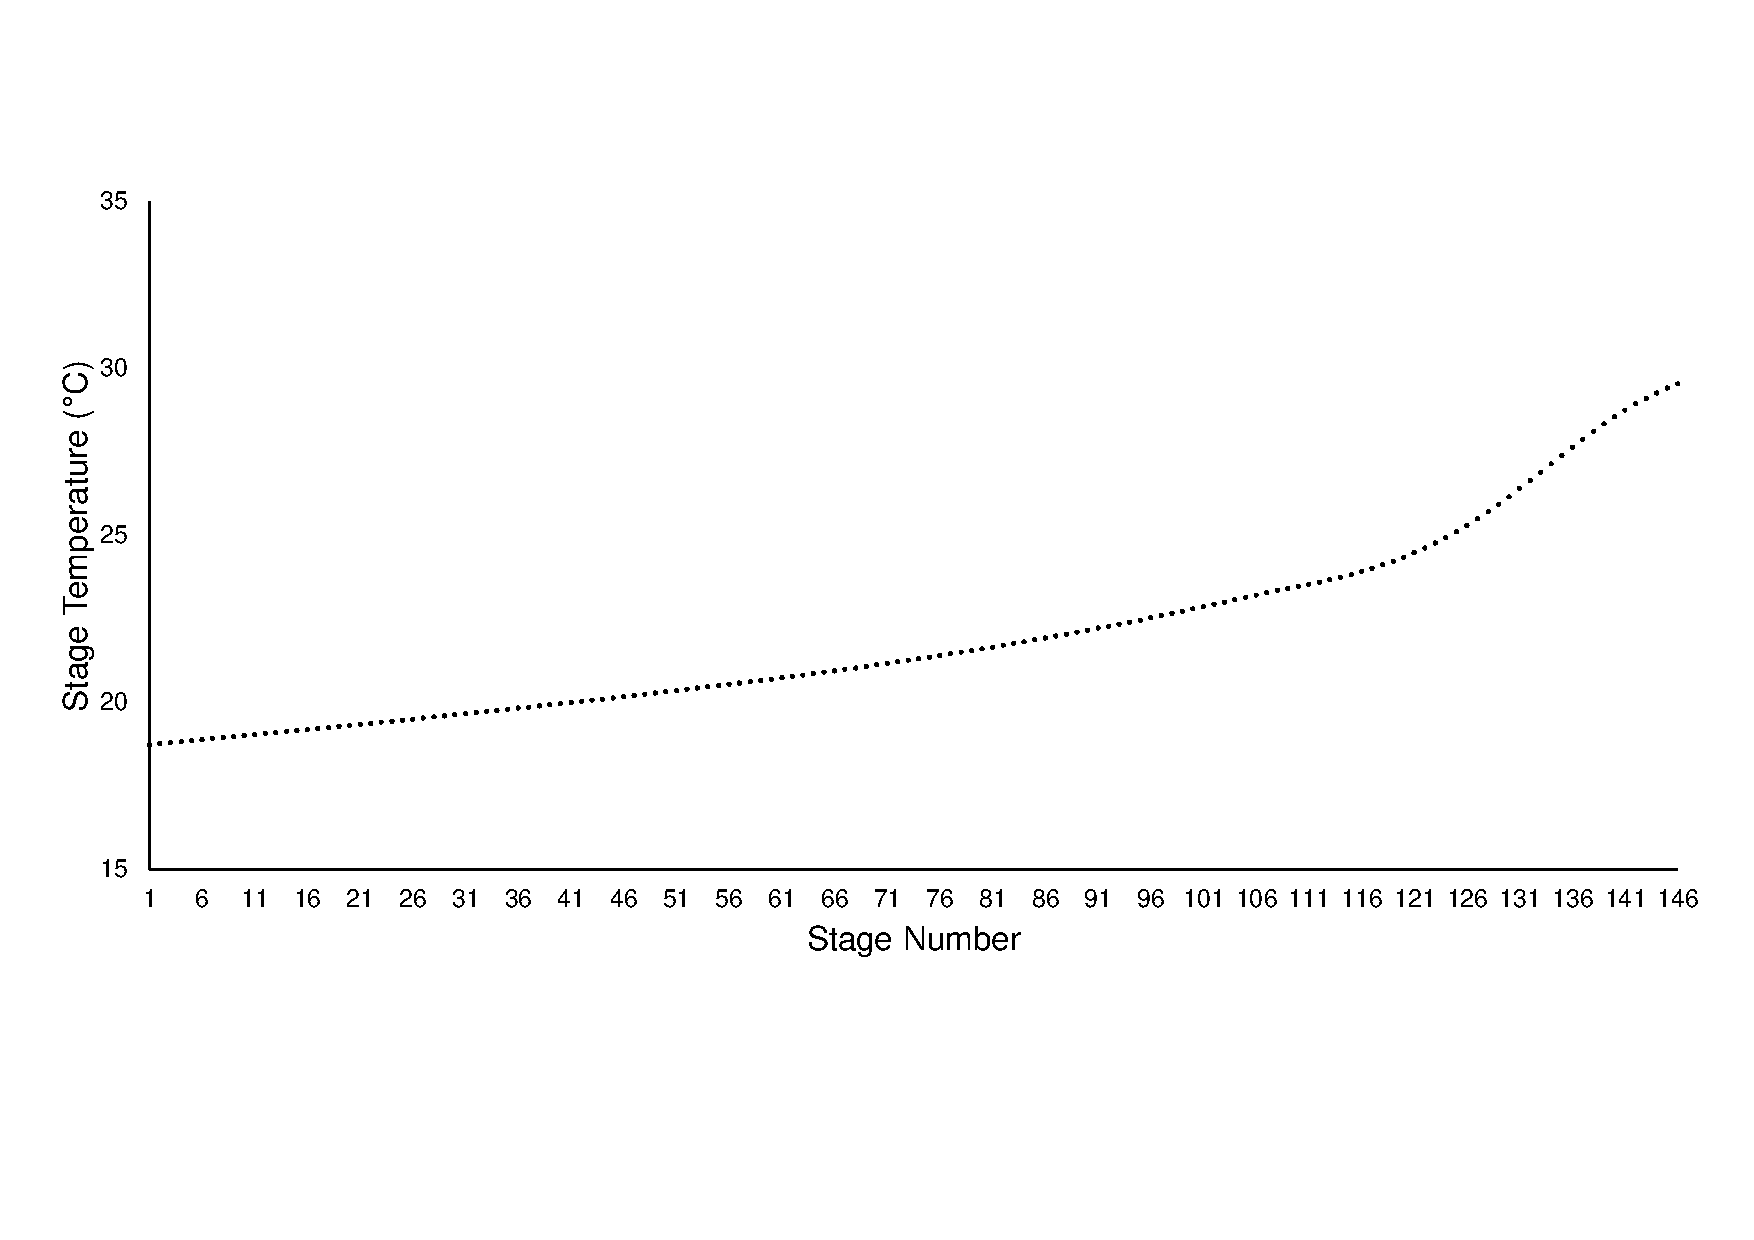
\includegraphics[width=1.0\textwidth]
    {c3-temperature-profile.pdf}}
\end{figure}

\begin{table}[htb]
    \centering
    \caption{CV Candidates for C3 Splitter composition indirect control.}
    \begin{tabular}{cc}
    \hline
    \textbf{Variable} (alias used in \mtc) & \textbf{Description} \\ \hline
     bf    & Bottoms to feed ratio \\
     vf    & Boilup to feed ratio \\
     lf    & Reflux to feed ratio \\
     rrcv  & Reflux ratio\\
     dfcv  & Distillate to feed ratio\\
     l     & Reflux rate $(kmol/h)$ \\
     v     & Boilup rate $(kmol/h)$ \\
     t8    & Stage 8 temperature   $(\celsius)$ \\
     t9    & Stage 9 temperature   $(\celsius)$ \\
     t10   & Stage 10 temperature  $(\celsius)$\\
     t11   & Stage 11 temperature  $(\celsius)$\\
     t12   & Stage 12 temperature  $(\celsius)$\\
     t129  & Stage 129 temperature $(\celsius)$\\
     t130  & Stage 130 temperature $(\celsius)$\\
     t131  & Stage 131 temperature $(\celsius)$\\
     t132  & Stage 132 temperature $(\celsius)$\\
     t133  & Stage 133 temperature $(\celsius)$\\
     t134  & Stage 134 temperature $(\celsius)$\\
     t135  & Stage 135 temperature $(\celsius)$\\
     t136  & Stage 136 temperature $(\celsius)$\\
    \hline
    \end{tabular}
    \label{tab:c3splittercvlist}
\end{table}

There are 20 CV candidates and 2 degrees of freedom for this case study. For a 
single measurement policy, for illustration purposes, there are 190 possible 
control structures (\autoref{eq:c3splitterpossible}), being clear the 
impracticability of evaluating all of these control structures manually. As 
stated before in the previous example, the problem becomes even larger if one
begins to consider linear combinations as CV candidates. 

\begin{equation}
    \binom{20!}{2!} = \frac{20!}{2!\times(20-2)!} = 190
    \label{eq:c3splitterpossible}
\end{equation}

With all preliminary information emphasized so far, it is possible to 
use the first tab of \mtc. Similarly as the first case study, the objective 
function, process constraints and CV candidates can be created at the 
``Function definitions'' panel, as can be seen in \Cref{fig:c3splitterload}. 
\Cref{fig:c3splitterloadvar} shows the variables being added to the *.mtc 
file, in order to be used for the study.

\begin{figure}[htb]
    \centering
    \caption{C3 Splitter Column Process - loading simulation. Process 
    constraint ``c2'' is multiplied by 4.184 to convert simulation reboiler 
    duty from $GCal/h$ to $GJ/h$.}
    \makebox[1.0\textwidth]{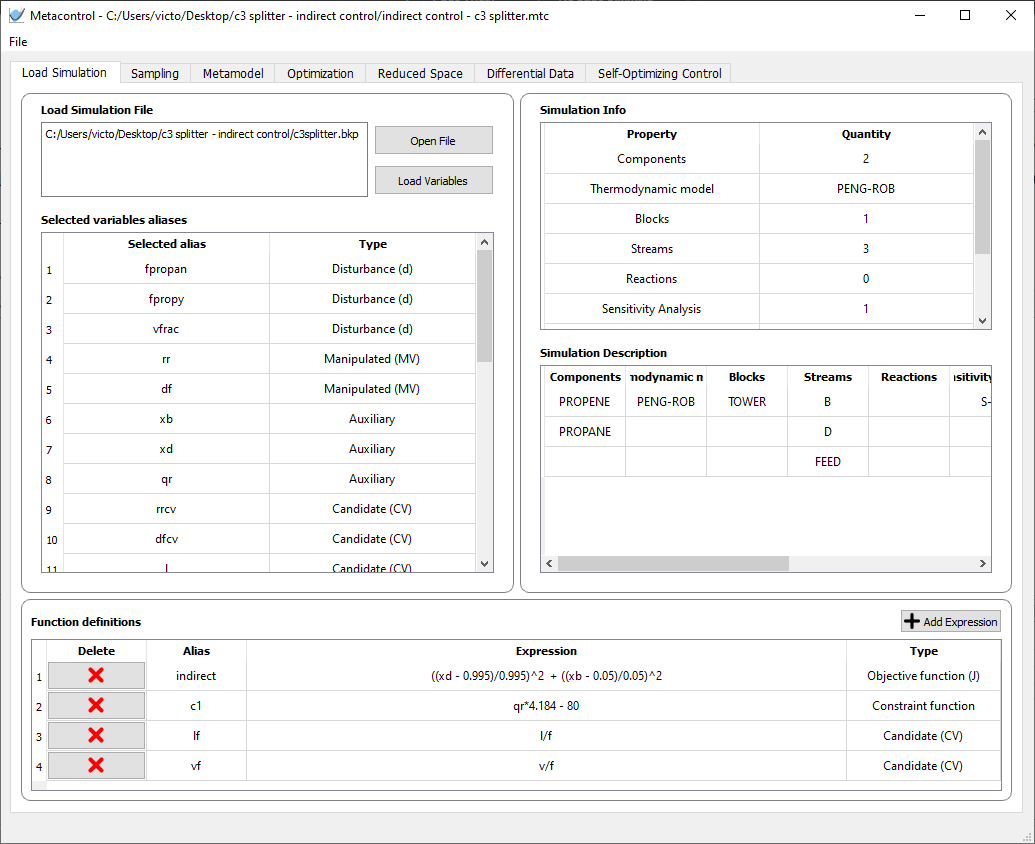
\includegraphics[width=1.0\textwidth]
    {c3splitter_load.PNG}}
    \label{fig:c3splitterload}
\end{figure}

\begin{figure}[htb]
    \centering
    \caption{C3 Splitter Column Process - loading variables from Aspen Plus.}
    \label{fig:c3splitterloadvar}
    \makebox[1.0\textwidth]{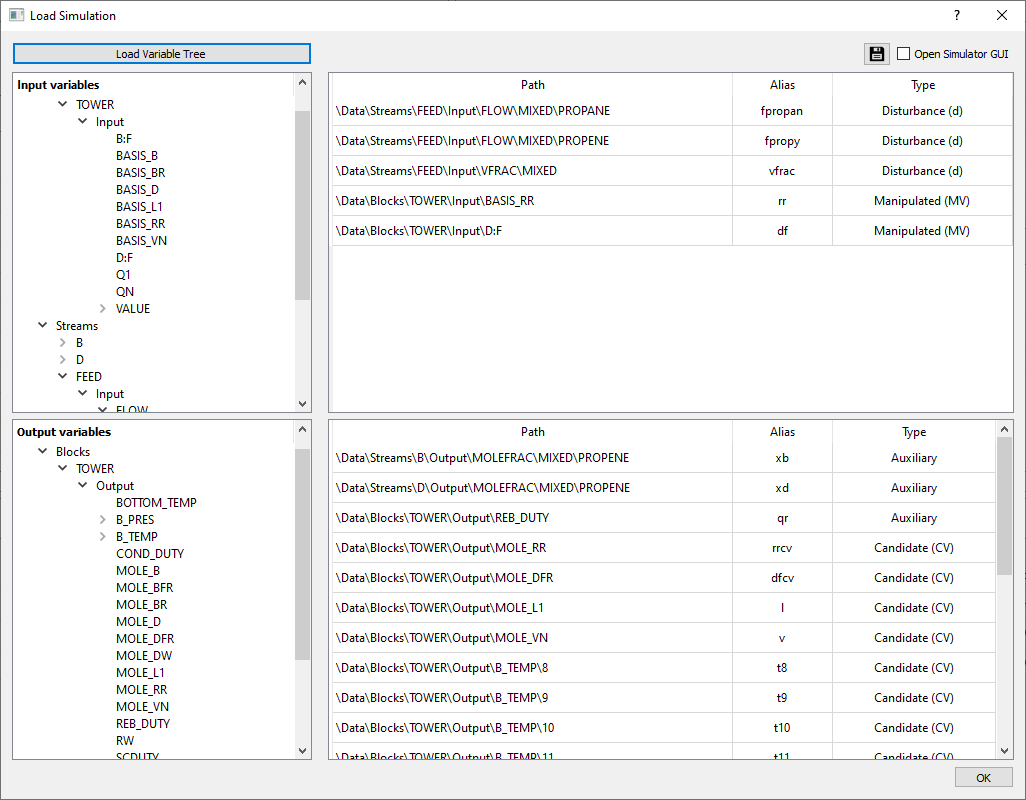
\includegraphics[width=1.0\textwidth]
    {c3splitter-load-variables.PNG}}
\end{figure}

For this case study, only 60 initial points were sampled. These points were 
refined by the algorithm from \textcite{Caballero2008} implemented in \mtc in 
order to find the optimal nominal operating point. Using a \textit{K-fold} 
validation metric, one of the features that are implemented in \mtc, it was 
found that using the quadratic regression polynomial yielded the most 
desirable metrics, as can be seen in 
\Cref{fig:c3splitterpoly0,,fig:c3splitterpoly2}. This is a valuable feature: 
it systematically informs, for the problem being studied, which regression 
model will yield the most accurate results.

\begin{figure}[htb]
    \centering
    \caption{K-fold validation metric for constant (poly0) regression model.}
    \label{fig:c3splitterpoly0}
    \makebox[1.0\textwidth]{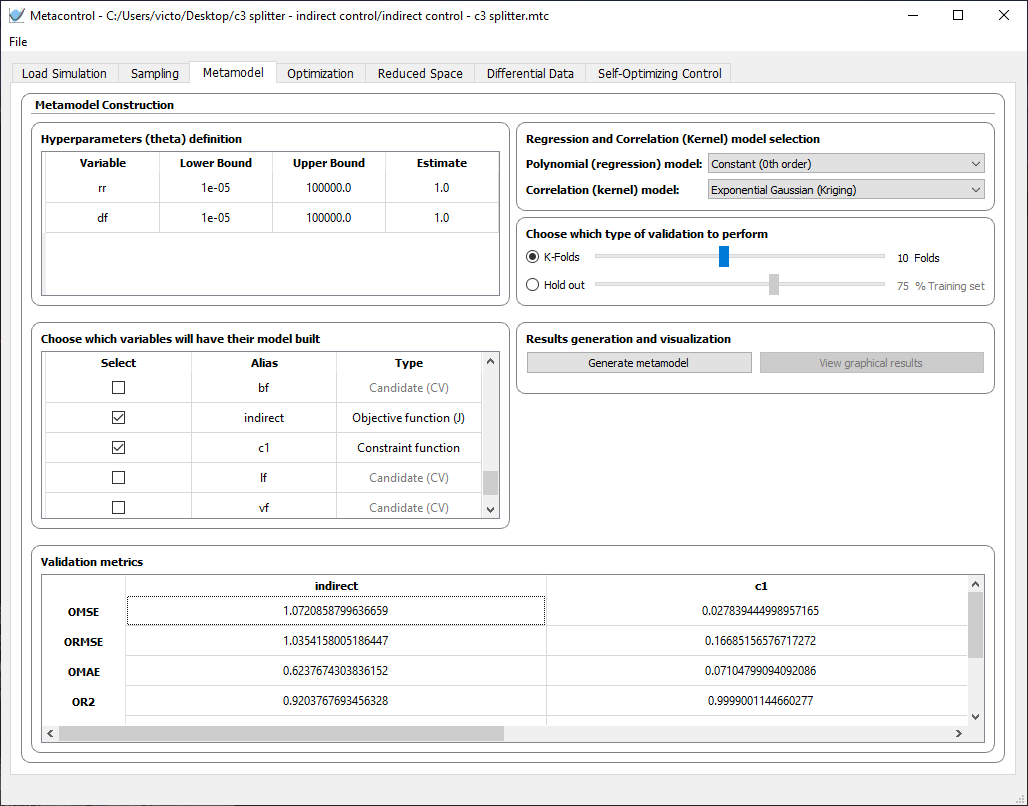
\includegraphics[width=1.0\textwidth]
    {c3splitterpoly0.PNG}}
\end{figure}

\begin{figure}[htb]
    \centering
    \caption{K-fold validation metric for linear (poly1) regression model.}
    \label{fig:c3splitterpoly1}
    \makebox[1.0\textwidth]{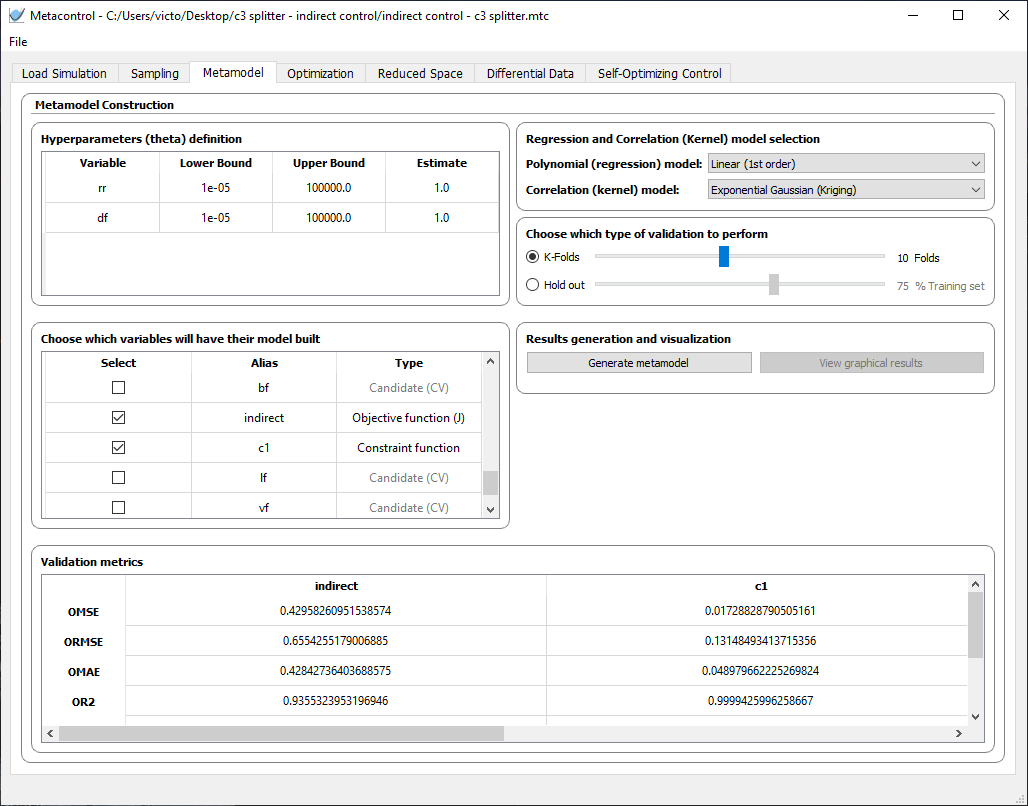
\includegraphics[width=1.0\textwidth]
    {c3splitterpoly1.PNG}}
\end{figure}

\begin{figure}[htb]
    \centering
    \caption{K-fold validation metric for quadratic (poly2) regression model.}
    \label{fig:c3splitterpoly2}
    \makebox[1.0\textwidth]{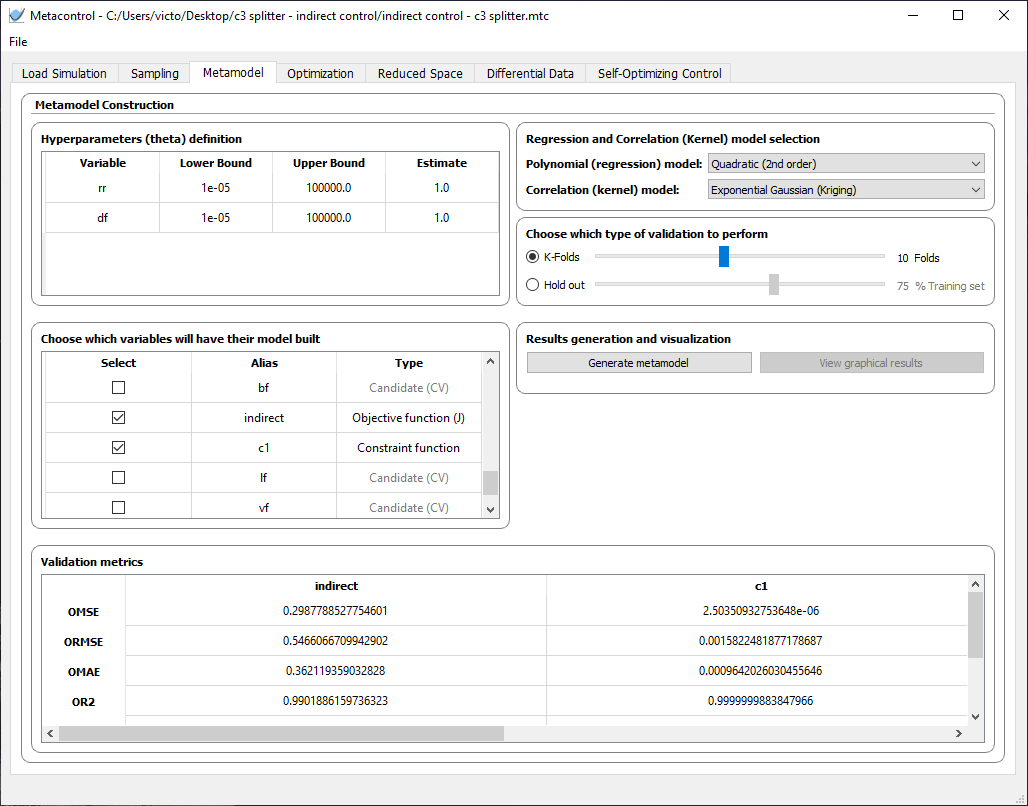
\includegraphics[width=1.0\textwidth]
    {c3splitterpoly2.PNG}}
\end{figure}

The optimization results found are described in \Cref{fig:c3splitteropt}. 
There are no active constraints for this problem, and therefore there are 2 
unconstrained degrees of freedom left for self-optimizing control purposes. 
The values for the decision variables are virtually the same ones found by 
\textcite{Alves2018}. This was expected since the direct control strucutre 
proposed came from an economic plantwide structure proposal (controlling 
propene distillate and bottoms compositions). The difference between the 
optimal decision variables values found previously by \textcite{Alves2018} 
and now, can be associated to the rounded setpoint of the composition of 
propene at the bottom stream.

An optimization was performed using the process simulator internal optimizer, 
to make the reader able to compare with the optimization using the surrogate 
model with the refinement algorithm from \textcite{Caballero2008}. As in the 
first case study, the results are nearly identical 
(\Cref{tab:c3splitter-optcomparison}).

\begin{figure}[htb]
    \centering
    \caption{Indirect control index objective function being minimized using 
    surrogate metamodel.}
    \label{fig:c3splitteropt}
    \makebox[1.0\textwidth]{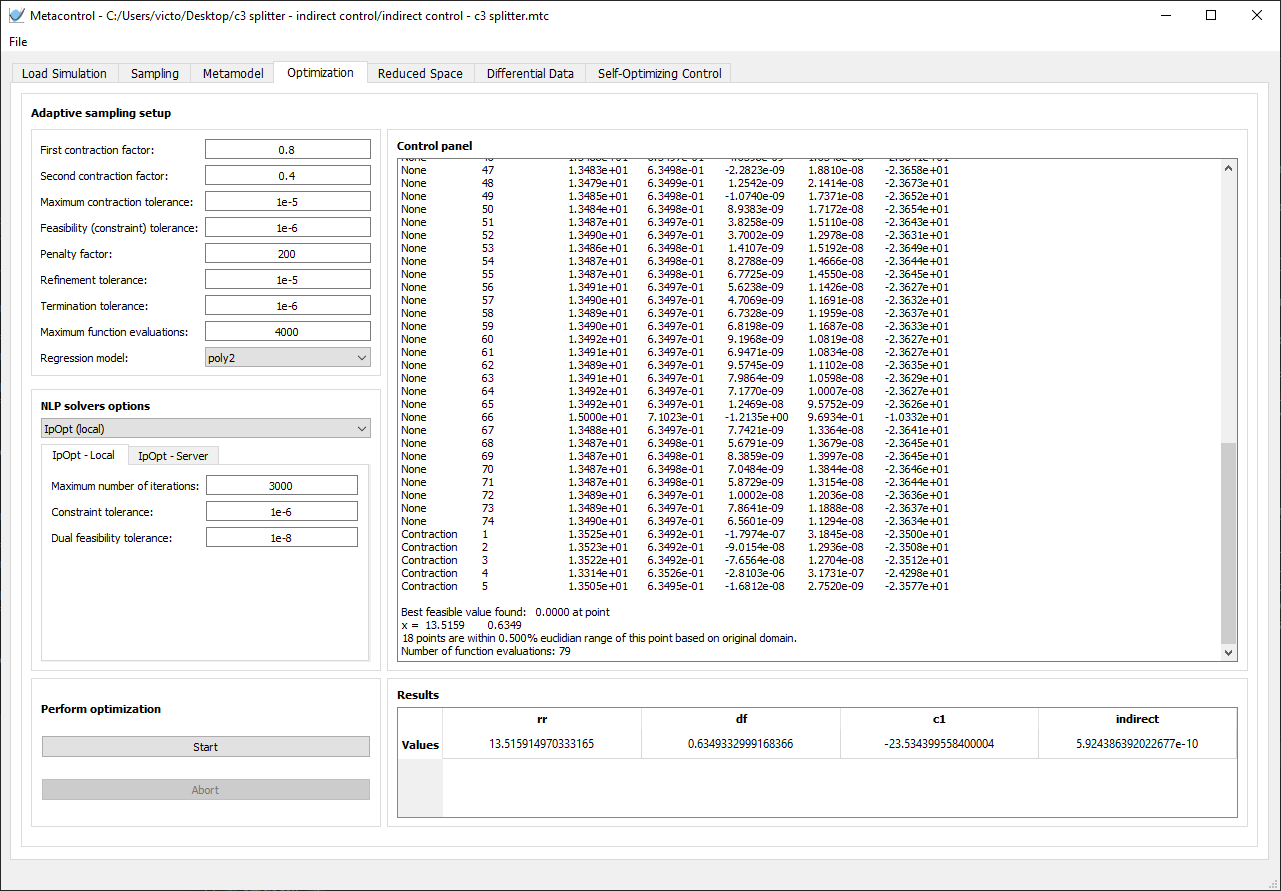
\includegraphics[width=1.0\textwidth]
    {c3splitter_caballero.PNG}}
\end{figure}

\begin{table}[htb]
		\centering
		\caption{Optimization runs: \textit{Aspen Plus vs Metacontrol} - Decision
		variables and objective function - C3 Splitter Indirect control}
		\resizebox{\textwidth}{!}{
		\begin{tabular}{c c c c}
	
			\hline
			 & Objective function ``indirect'' & Reflux Ratio & 
			Distillate to feed ratio \\
			\hline
			Aspen Plus & $ 7.47 \times 10^{-15} $ & 13.5246 & 0.6349 \\
			\mtc & $ 5.92 \times 10^{-10} $ & 13.5159 & 0.6349 \\
			\hline
		\end{tabular}
		}
		\label{tab:c3splitter-optcomparison}
\end{table}

As stated before, 20 CV candidates were chosen to be tested by \mtc. 
Differently from the first case study, where it was used the *.csv import 
feature (merely to show the capability of the software), on this example the 
reduced space problem sampling was done internally in \mtc. 
Since there are no active constraints, the same *.bkp file can be used (i.e. It 
is not necessary to implement any design specifications to consume the degrees 
of freedom for active constraints). 

\Cref{fig:c3splitterredspace} shows the 
interface built to select the reduced space problem simulation file, where the 
user can simply point to the *.bkp file using the GUI and the sampling assistant 
will use the limits that were imposed under the ``Range of disturbances'' panel 
in order to generate the data for the reduced space problem. The latter can be 
inspected in \Cref{fig:c3splitterredspace-file}.
\nomenclature[A]{GUI}{Graphical User Interface}

\begin{figure}[htb]
    \centering
    \caption{Reduced space problem - sampling using a .*bkp file.}
    \label{fig:c3splitterredspace}
    \makebox[1.0\textwidth]{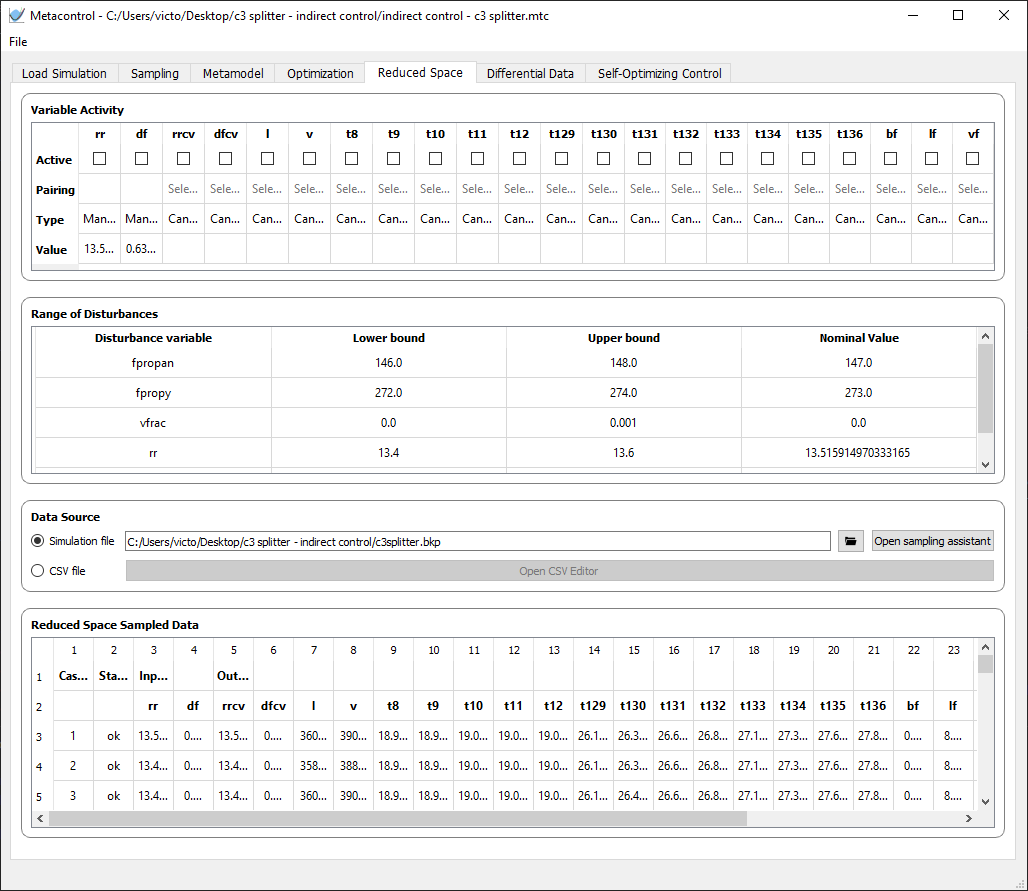
\includegraphics[width=1.0\textwidth]
    {c3splitter-reduced-space.PNG}}
\end{figure}

\begin{figure}[htb]
    \centering
    \caption{Reduced space problem - pointing the .*bkp file location.}
    \label{fig:c3splitterredspace-file}
    \makebox[1.0\textwidth]{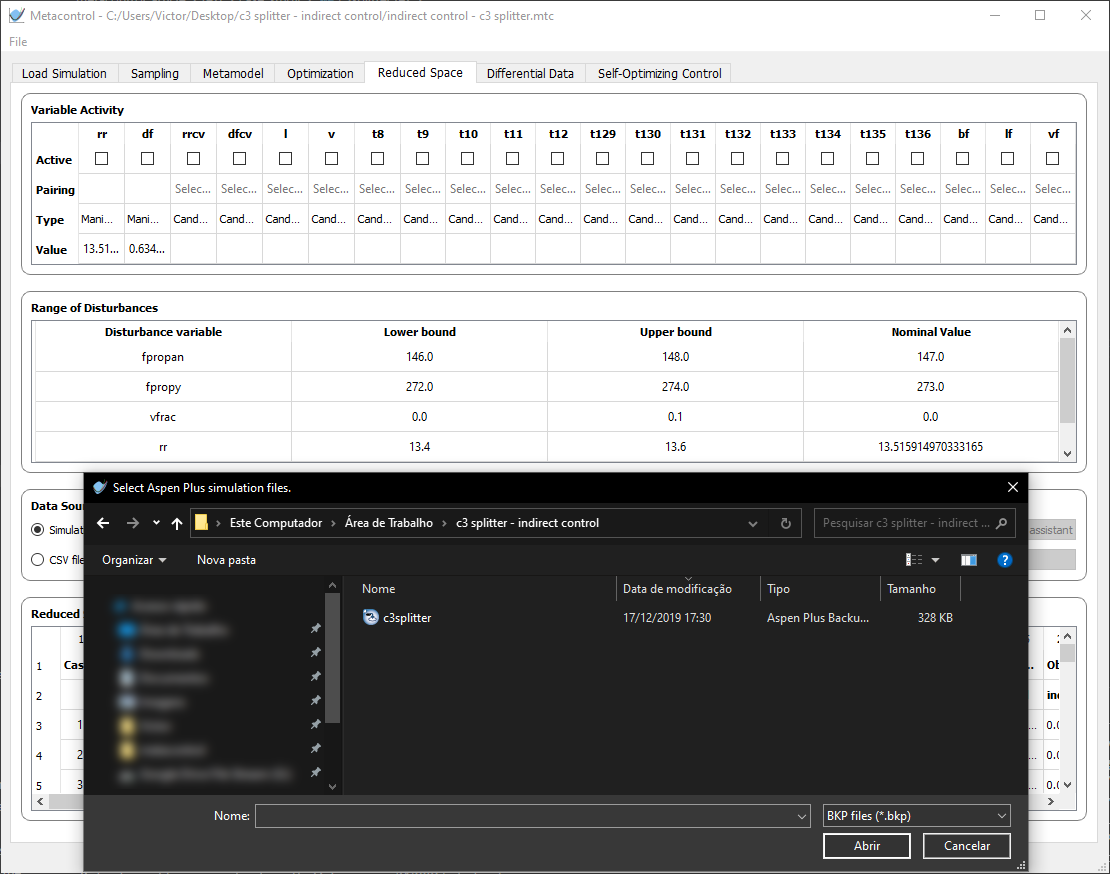
\includegraphics[width=1.0\textwidth]
    {c3splitter-point-file.PNG}}
\end{figure}

\begin{figure}[htb]
    \centering
    \caption{Reduced space problem - Sampling assistant: Identical to the 
    Sampling Assistant that exists under the ``Sampling'' tab, in order to keep 
    consistency of interface across \mtc. Number 1 indicates the button to 
    open the Assistant, 2 consists in the main screen, 3 is the button that 
    opens the settings of the sampling technique that will generate the input 
    data; 4 generates the data. In addition, number 5 depicts the control of 
    the sampling procedure: Sample data, cancel, close screen (``Done'' 
    button). Lastly, the user can abort the sampling at any time using the 
    ``Abort'' button (number 6) or export the design of experiments as a 
    *.csv (number 7).}
    \label{fig:c3splitterredspace-file}
    \makebox[1.0\textwidth]{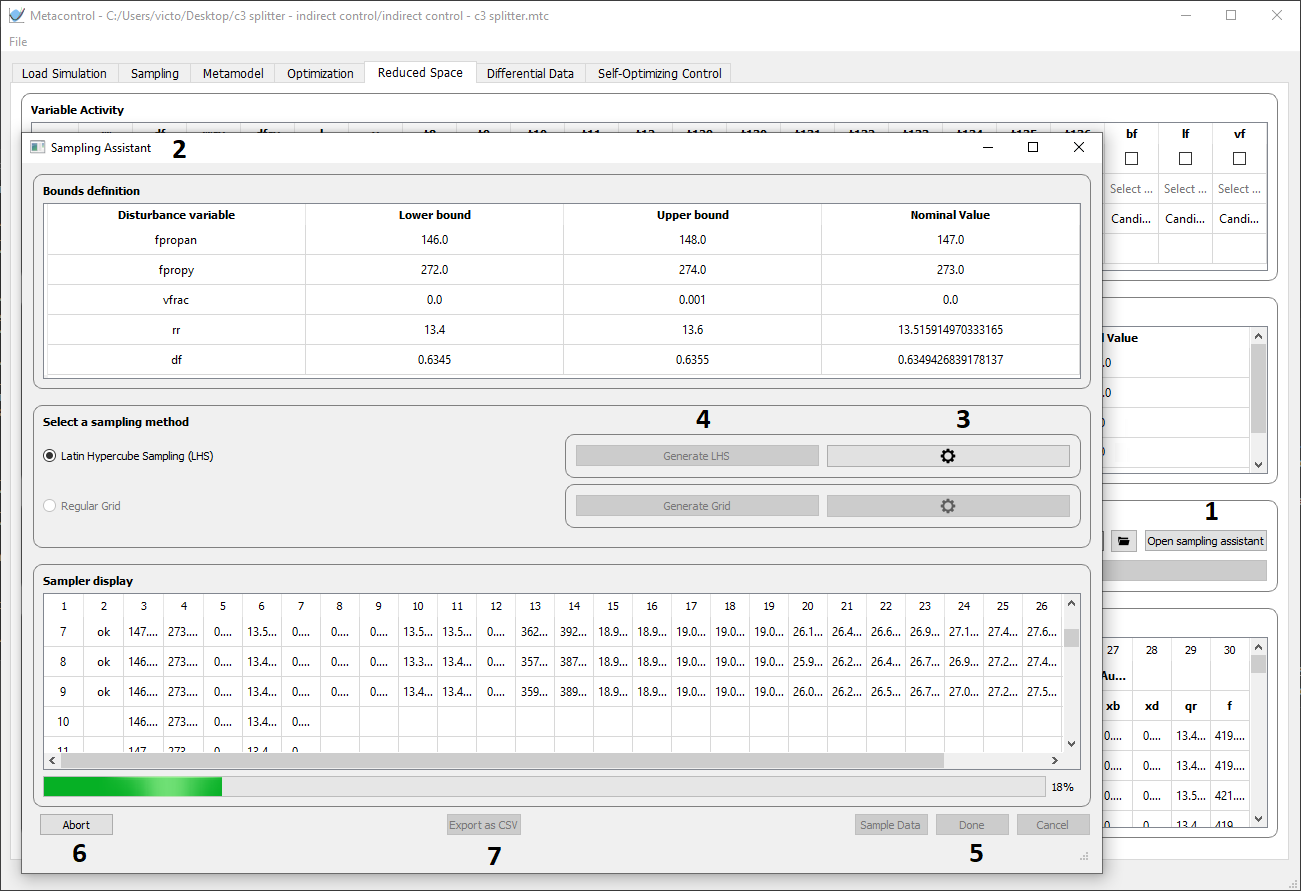
\includegraphics[width=1.0\textwidth]
    {c3splitter-redspace-sampling.PNG}}
\end{figure}

Using the sampled data from the simulation file, the user can go to 
``Differential Data'' tab and generate the gradients and the hessians, exactly 
as done at the first case study. \Cref{fig:c3splittergrad} shows the 
gradients $G^y, G^y_{d}$ and the hessians $J_{uu}, J_{ud}$ calculated using 
\mtc.

\begin{figure}[htb]
    \centering
    \caption{``Differential Data'' tab - C3 Splitter indirect control.}
    \label{fig:c3splittergrad}
    \makebox[1.0\textwidth]{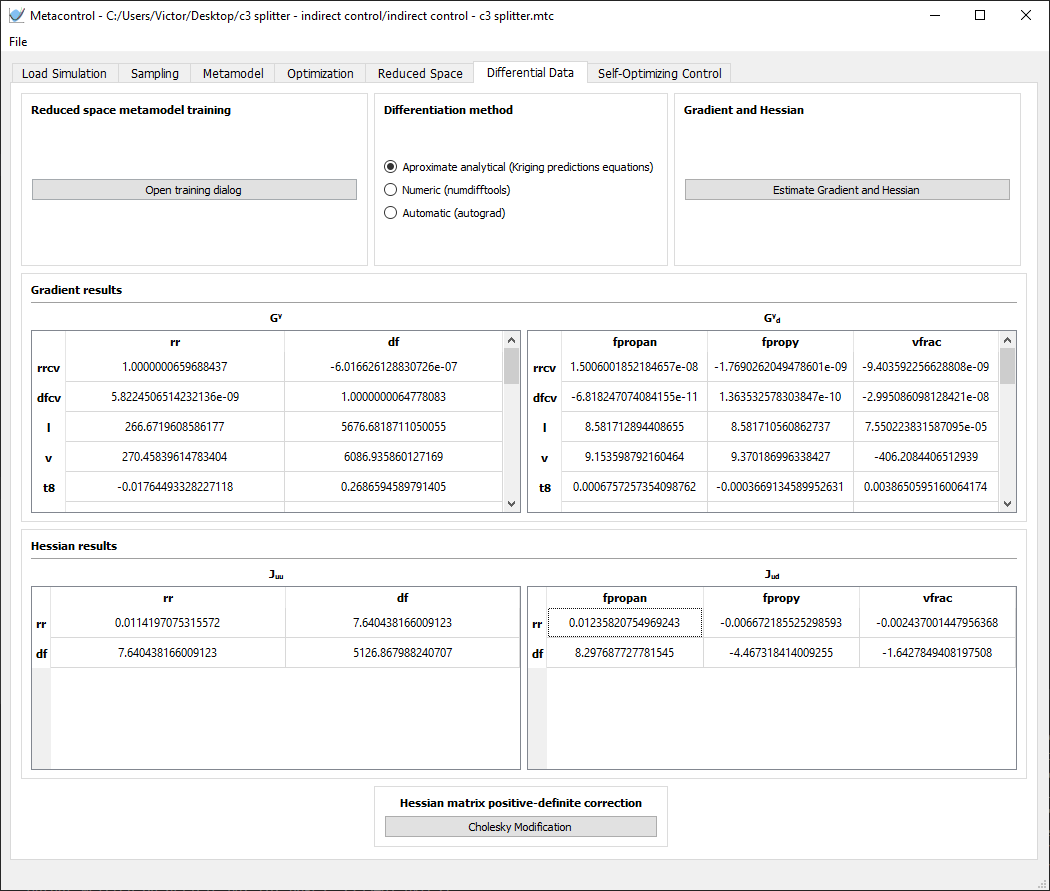
\includegraphics[width=1.0\textwidth]
    {c3splitter-gradients.PNG}}
\end{figure}

Similarly to the first case study, the gradients obtained by \mtc were 
compared against the ones generated by the process simulator. Not surprisingly, 
they were virtually identical, which is an evidence of the robustness of the 
previously proposed methodology \textcite{Alves2018} that is embedded in the 
\mtc software. 

\FloatBarrier  % to force the table to start on top of page
\small
\setlength\LTleft{0cm}
\setlength\LTright{0cm}
\begin{longtable}{ccc}
    %first page header and caption
    \caption{High-order data obtainment: \textit{Aspen Plus vs Metacontrol} - 
    C3 Splitter column case study.}\label{tab:c3splittergrads}\\
    \hline
        & $G^{y}$ & $G_{d}^y$ \\*
    \hline
    \\
    \endfirsthead

    % continuation headers and caption
    \caption[]{(continued)}\\
    \hline
        & $G^{y}$ & $G_{d}^y$ \\
    \hline
    \endhead

    % rows data here
    \rotatebox[origin=c]{90}{\mtc} & $
    \begin{bmatrix}
        \num{1.00000000334231}      & \num{-1.60837442689474e-06} \\
        \num{1.53803848277547e-10}  & \num{0.999999989514324}     \\
        \num{266.671973137410}      & \num{5676.68329936300}      \\
        \num{270.458753978942}      & \num{6086.94361132937}      \\
        \num{-0.0177001378556690}   & \num{0.270006308409754}     \\
        \num{-0.0188866192712895}   & \num{0.289384248637259}     \\
        \num{-0.0200939793580083}   & \num{0.309351100081970}     \\
        \num{-0.0213221458452405}   & \num{0.329926416199304}     \\
        \num{-0.0225718144631595}   & \num{0.351139981309695}     \\
        \num{0.0527183703992920}    & \num{74.2427939801773}      \\
        \num{0.0613151357019541}    & \num{76.6816022260870}      \\
        \num{0.0691092102696593}    & \num{78.3864475354819}      \\
        \num{0.0758510487705565}    & \num{79.2567344474355}      \\
        \num{0.0812928015068666}    & \num{79.2232500217448}      \\
        \num{0.0852659903216080}    & \num{78.2564452291187}      \\
        \num{0.0876531822344054}    & \num{76.3710096854737}      \\
        \num{0.0890627871441921}    & \num{73.6323803514866}      \\
        \num{-1.53803855527242e-10} & \num{-0.999999989514330}    \\
        \num{0.634933313482458}     & \num{13.5159135056456}      \\
        \num{0.643949541588581}     & \num{14.4927667602665}
    \end{bmatrix}
    $ & 
    $
    \begin{bmatrix}
        \num{-3.29856328237313e-09} & \num{1.25000581675374e-09}  & \num{-9.56790032742503e-08} \\
        \num{-6.12195123602312e-11} & \num{4.54312002598694e-12}  & \num{9.72792760940055e-10}  \\
        \num{8.58171741161802}      & \num{8.58171180678352}      & \num{-2.60618905111412e-05} \\
        \num{9.15358128168813}      & \num{9.37015609215126}      & \num{-406.208917666402}     \\
        \num{0.000678261840569012}  & \num{-0.000367323094241650} & \num{0.00381067428315477}   \\
        \num{0.000726938310732710}  & \num{-0.000393713138107657} & \num{0.00408496100005842}   \\
        \num{0.000777107336637297}  & \num{-0.000420905292822426} & \num{0.00436686559738872}   \\
        \num{0.000828820701764815}  & \num{-0.000448875223750798} & \num{0.00465782074138010}   \\
        \num{0.000882087335946104}  & \num{-0.000477740521013113} & \num{0.00495687721940721}   \\
        \num{0.125653757087539}     & \num{-0.0678253909169260}   & \num{0.0585547203808428}    \\
        \num{0.129125788540487}     & \num{-0.0696777290719591}   & \num{0.0507483925614849}    \\
        \num{0.131391990089653}     & \num{-0.0708790346941915}   & \num{0.0428859830193394}    \\
        \num{0.132297232636472}     & \num{-0.0713469276140274}   & \num{0.0351065558884792}    \\
        \num{0.131738960125607}     & \num{-0.0710260484876851}   & \num{0.0275867248881152}    \\
        \num{0.129678763765447}     & \num{-0.0698971580401931}   & \num{0.0204757879086981}    \\
        \num{0.126149146999142}     & \num{-0.0679786282240887}   & \num{0.0139115782309413}    \\
        \num{0.121428936865429}     & \num{-0.0653838235368392}   & \num{0.0104362697621862}    \\
        \num{6.12195055552325e-11}  & \num{-4.54312606595640e-12} & \num{-9.72792956069799e-10} \\
        \num{-5.00480259906448e-10} & \num{-1.16413727666999e-09} & \num{-7.10204203949764e-08} \\
        \num{-0.000335194773108412} & \num{0.000180485520047226}  & \num{-0.967164338893723} 
    \end{bmatrix}
    $ \\
    \\
    \hline
    \\
    \rotatebox[origin=c]{90}{Aspen Plus} & $
    \begin{bmatrix}
        \num{1}                     & \num{0}                  \\ 
        \num{8.25100000000000e-19}  & \num{1}                  \\ 
        \num{266.672000000000}      & \num{5676.68400000000}   \\ 
        \num{270.459000000000}      & \num{6086.95300000000}   \\ 
        \num{-0.0176510000000000}   & \num{0.268892700000000}  \\
        \num{-0.0188340000000000}   & \num{0.288193700000000}  \\
        \num{-0.0200376000000000}   & \num{0.308083300000000}  \\
        \num{-0.0212623000000000}   & \num{0.328581200000000}  \\
        \num{-0.0225082000000000}   & \num{0.349707400000000}  \\
        \num{0.0561285000000000}    & \num{74.1791600000000}   \\
        \num{0.0643842000000000}    & \num{76.6318200000000}   \\
        \num{0.0717863000000000}    & \num{78.3507500000000}   \\
        \num{0.0780960000000000}    & \num{79.2344000000000}   \\
        \num{0.0831061000000000}    & \num{79.2129400000000}   \\
        \num{0.0866598000000000}    & \num{78.2562800000000}   \\
        \num{0.0886649000000000}    & \num{76.3784900000000}   \\
        \num{0.0891023000000000}    & \num{73.6377200000000}   \\
        \num{-4.78600000000000e-17} & \num{-1}                 \\
        \num{0.634933300000000}     & \num{13.5159100000000}   \\
        \num{0.643949900000000}     & \num{14.4927400000000}
    \end{bmatrix}
    $ & 
    $
    \begin{bmatrix}
        \num{0}                     & \num{0}                     & \num{0}                     \\
        \num{1.51160000000000e-07}  & \num{1.51160000000000e-07}  & \num{0}                     \\
        \num{8.58170400000000}      & \num{8.58170400000000}      & \num{0}                     \\
        \num{9.15356900000000}      & \num{9.37014800000000}      & \num{-406.209500000000}     \\
        \num{0.000678086000000000}  & \num{-0.000365120000000000} & \num{0.00384634000000000}   \\
        \num{0.000726758000000000}  & \num{-0.000391330000000000} & \num{0.00412243000000000}   \\
        \num{0.000776915000000000}  & \num{-0.000418340000000000} & \num{0.00440693000000000}   \\
        \num{0.000828606000000000}  & \num{-0.000446170000000000} & \num{0.00470014000000000}   \\
        \num{0.000881882000000000}  & \num{-0.000474860000000000} & \num{0.00500234000000000}   \\
        \num{0.126061800000000}     & \num{-0.0678794000000000}   & \num{0.0650386000000000}    \\
        \num{0.129518400000000}     & \num{-0.0697406000000000}   & \num{0.0567382000000000}    \\
        \num{0.131761200000000}     & \num{-0.0709483000000000}   & \num{0.0482816000000000}    \\
        \num{0.132635700000000}     & \num{-0.0714192000000000}   & \num{0.0398446000000000}    \\
        \num{0.132040500000000}     & \num{-0.0710987000000000}   & \num{0.0316179000000000}    \\
        \num{0.129939200000000}     & \num{-0.0699672000000000}   & \num{0.0237940000000000}    \\
        \num{0.126367100000000}     & \num{-0.0680438000000000}   & \num{0.0165530000000000}    \\
        \num{0.121430200000000}     & \num{-0.0653854000000000}   & \num{0.0100492000000000}    \\
        \num{8.69120000000000e-08}  & \num{8.69120000000000e-08}  & \num{-4.35600000000000e-17} \\
        \num{2.04306000000000e-06}  & \num{2.04306000000000e-06}  & \num{0}                     \\
        \num{-0.000332970000000000} & \num{0.000182695000000000}  & \num{-0.967165500000000} 
    \end{bmatrix}
    $ \\
    \\
    \hline

\end{longtable}

\begin{table}[htb]
	\centering
    \caption{Mean-squared error of high-order data obtainment: 
    \textit{Aspen Plus vs Metacontrol} - C3 Splitter column}	
	\begin{tabular}{l l l}
	\hline
	 & $G^{y}$ & $G_{d}^y$ \\ \hline
	 Mean-squared error & \num{1.6738e-05} & \num{3.1706e-08} \\ \hline
	\end{tabular}
	\label{tab:c3splittermsegrad}
\end{table}

From \Cref{tab:c3splittergrads} it is shown that the gradients generated 
using the metamodels built by \mtc are extremely close to the evaluation of 
the gradients directly using the nonlinear model from the process simulator.

Since all required high-order data it is available, the user can go to the 
last step of the top-down procedure, which consists in the loss evaluation 
for the control structures with \soc properties. The last required 
information consists of the disturbances and measurement error matrices. 
Similarly as \textcite{Alves2018}, $10\%$ of the nominal feed component 
flow rates were considered as the expect magnitudes, and for the feed vapor 
fraction it was also considered a $10\%$ disturbance magnitude 
(\Cref{eq:wdc3}). Regarding the measurement errors, for flows and flow 
ratios, the authors considered a $0.001$ magnitude representing the 
accuracy of flow meters. For temperature measurements, $0.5\celsius$, a 
value that can realistically represent thermocouples and RTD sensors 
accuracies (both are typically used in the industry, specially 
distillation), was used. The order of \Cref{eq:wdc3,,eq:wnyc3} are the 
same from the \mtc user interface: An alphabetical order of the aliases 
given at the first tab. The insertion of all information regarding the 
magnitude matrices can be seen in \Cref{fig:c3splittersocinput}.

\begin{equation}
	W_{d} = diag(14.7, 27.3, 0.1)
	\label{eq:wdc3}
\end{equation}

\begin{equation}
    \begin{split}
        W_{n}^{y} = diag(0.001,0.001,0.001,0.001,0.001,0.5,0.5,0.5,0.5,0.5,0.5,\\
        0.5,0.5,0.5,0.5,0.5,0.5,0.5,0.001,0.001)
        \label{eq:wnyc3}
    \end{split}
\end{equation}

\begin{figure}[htb]
    \centering
    \caption{Input screen in \mtc ``\soc'' tab - C3 Splitter column: Here, all 
    190 possible control structures for a single measurement policy were 
    considered to be evaluated by \mtc. For linear combinations of 
    measurements as CV candidates, the 50 best ones of each possible 
    subset size were evaluated, when possible. For subset sizes of 19 and 
    20, all combinations were considered (20 and 1, respectively).}
    \label{fig:c3splittersocinput}
    \makebox[1.0\textwidth]{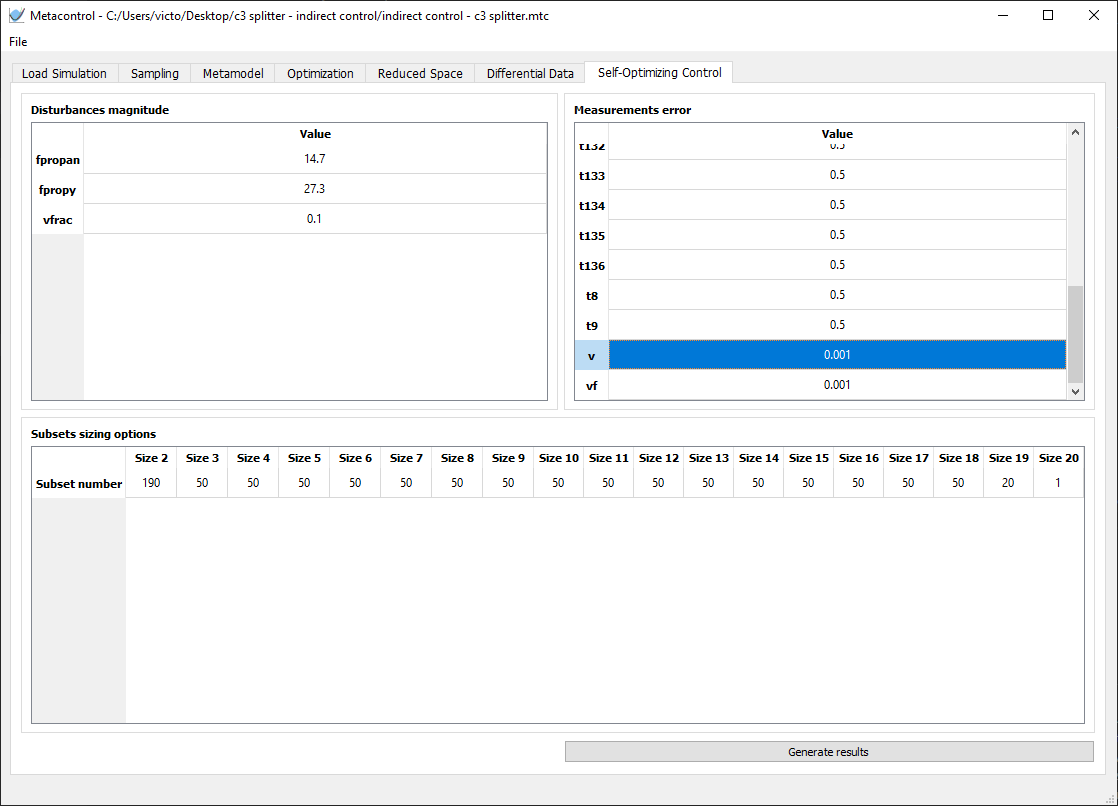
\includegraphics[width=1.0\textwidth]
    {c3splittersocinput.PNG}}
\end{figure}

Clicking on ``Generate results'' button, the user can inspect the number of 
best control structures that he entered in the previous screen. Analyzing 
\Cref{fig:c3cvgood}, one can easily see that controlling sensitive 
temperatures associated together with flows and flow ratios generates a 
control strucutre capable of indirect controlling both distillate and bottom 
streams compositions with a small incurred loss. On the other hand, stages 
with small temperatures deviation between them gave unacceptable losses, 
similarly as found by different authors \textcite{Alves2018,Hori2007}, for 
instance. The latter result can be found in \Cref{fig:c3cvtempbad}. 
More generally, this result is also a confirmation that the slope criterion 
from \textcite{Luyben2006} it is a good starting assumption when one
it is deciding which variable should be controlled. The main difference when 
one is using \soc is that the mathematical formulation derived by the 
authors of the technology already translated desired robust control and 
near-optimal operation from a heuristic and qualitative perspective to 
a mathematical one, making the whole procedure systematic.

\begin{figure}[htb]
    \centering
    \caption{Best control structures for single measurement policy: Stages 
    with significant temperature deviation between them associated with 
    flow and flow ratios - namely boilup, reflux, boilup to feed ratio and 
    reflux to feed ratio.}
    \label{fig:c3cvgood}
    \makebox[1.0\textwidth]{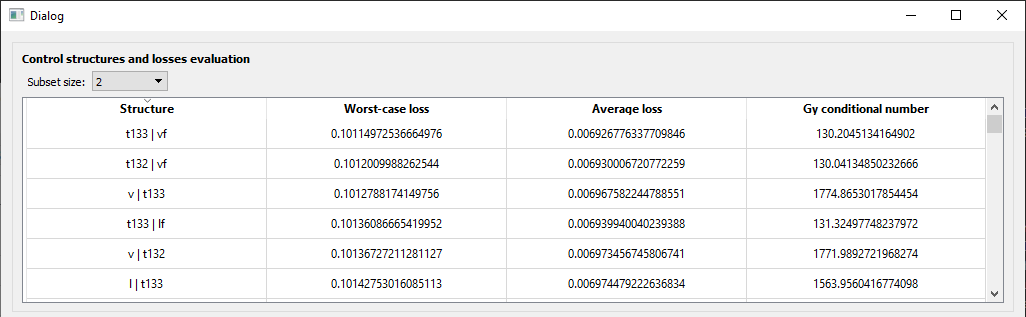
\includegraphics[width=1.0\textwidth]
    {c3splitter-good-cvs-size-2.PNG}}
\end{figure}

\begin{figure}[htb]
    \centering
    \caption{Worst control structures for single measurement policy using 
    exclusively temperature measurements: Stages with small temperature 
    deviation between them. One can easily note that the inspection of the 
    best and worst control structures is simple in \mtc: The user is capable 
    of sorting, using the graphical user interface built, the control 
    structures in ascending or descending order of worst-case loss, 
    average-case loss and conditional number.}
    \label{fig:c3cvtempbad}
    \makebox[1.0\textwidth]{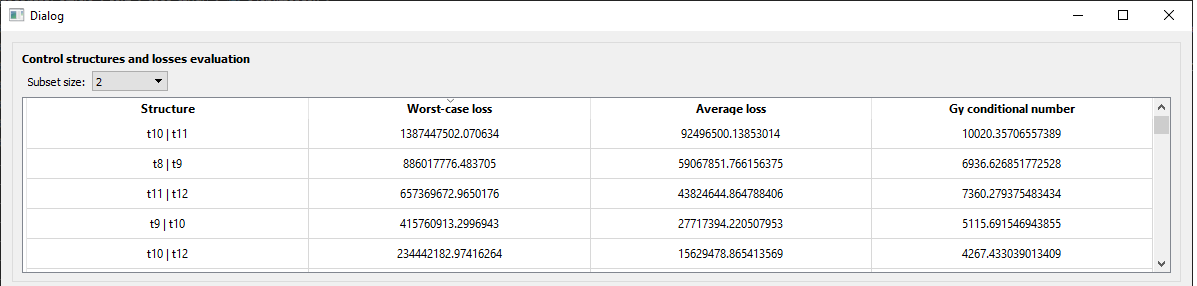
\includegraphics[width=1.0\textwidth]
    {c3splitter-bad-cvs-size-2-ts.PNG}}
\end{figure}


The analysis of the incurred loss when one is using linear combinations of 
measurements as CV candidates can be inspected in 
\Cref{fig:c3ss3,,fig:c3ss9}, and the usage of all measurements is depicted in 
\Cref{fig:c3ssall}. As stated by \textcite{Kariwala2008}, the usage of all 
available measurements it is often not necessary. Actually, a good tradeoff 
between the number of measurements used and the value of the loss generally 
exists in most cases. For instance, the worst-case loss when one uses all 
20 measurements is  approximately 0.0126 (\Cref{fig:c3ssall}), while using a 
simpler combination of 9 measurements gives a worst-case loss of 0.0141, 
only  approximately $11.9 \%$ higher, but with less measurements forming the 
linear combination.

\begin{figure}[htb]
    \centering
    \caption{Best control structures using linear combinations of measurements 
    as CV candidates - Subset of size 3.}
    \label{fig:c3ss3}
    \makebox[1.0\textwidth]{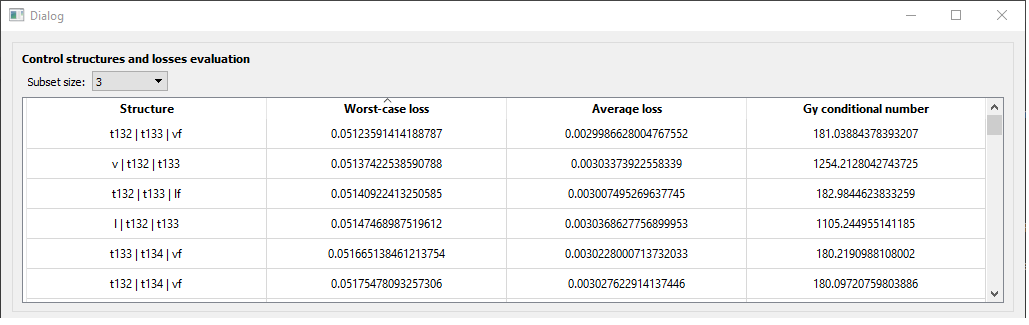
\includegraphics[width=1.0\textwidth]
    {c3splitter-good-cvs-size-3.PNG}}
\end{figure}

\begin{figure}[htb]
    \centering
    \caption{Best control structures using linear combinations of measurements 
    as CV candidates - Subset of size 6.}
    \label{fig:c3ss6}
    \makebox[1.0\textwidth]{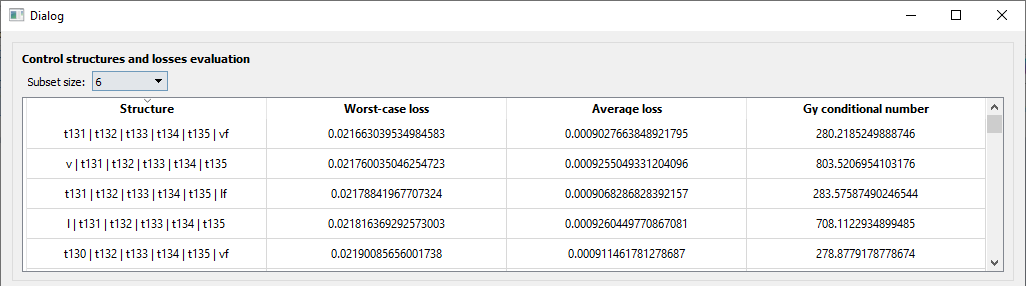
\includegraphics[width=1.0\textwidth]
    {c3splitter-good-cvs-size-6.PNG}}
\end{figure}

\begin{figure}[htb]
    \centering
    \caption{Best control structures using linear combinations of measurements 
    as CV candidates - Subset of size 9.}
    \label{fig:c3ss9}
    \makebox[1.0\textwidth]{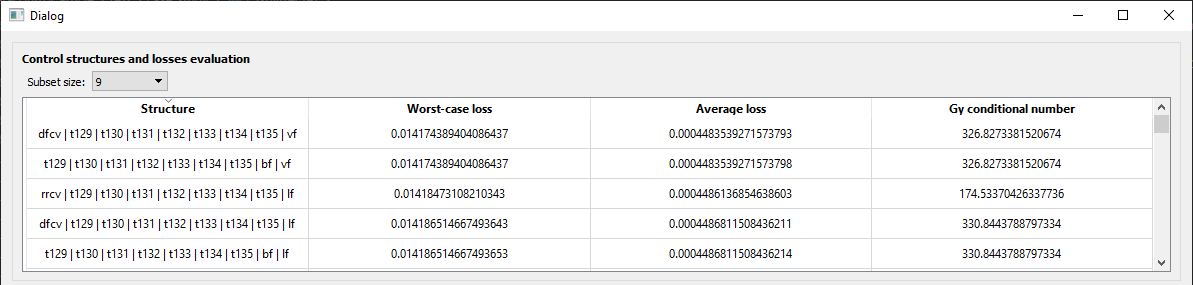
\includegraphics[width=1.0\textwidth]
    {c3splitter-good-cvs-size-9.PNG}}
\end{figure}

\begin{figure}[htb]
    \centering
    \caption{Best control structures using linear combinations of measurements 
    as CV candidates - All available measurements.}
    \label{fig:c3ssall}
    \makebox[1.0\textwidth]{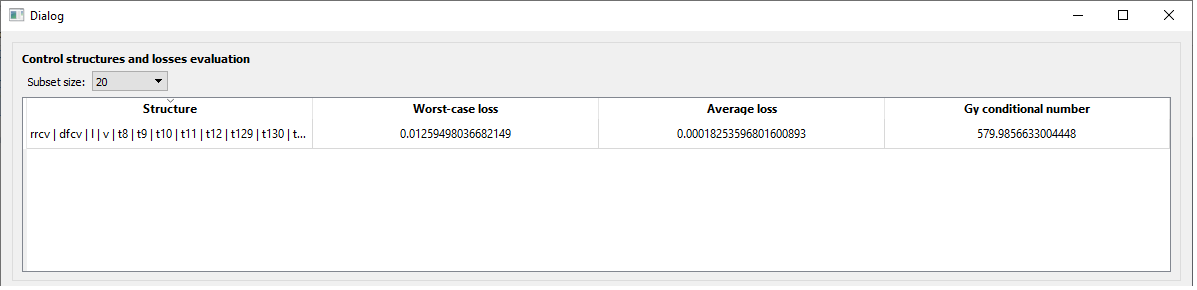
\includegraphics[width=1.0\textwidth]
    {c3splitter-good-cvs-size-all.PNG}}
\end{figure}

\FloatBarrier

\end{document}